\chapter{Desenvolvimento}
  
\section{O funcionamento do termistor}
 
	O termistor é um resistor variável à temperatura, característica pela qual seu nome é inspirado (temperatura + resistor), geralmente compostos por uma liga que contém cerâmica e outros polímeros. Suas aplicações mais habituais costumam acontecer em circuitos de monitoramento e controle de temperatura ou como limitador de corrente de partida. São separados, basicamente, em duas categorias:
	\begin{itemize}
		\item NTC (Negative Temperature Coefficient): São termistores que diminuem a sua resistência à medida em que a temperatura aumenta; E
		\item PTC (Positive Temperature Coefficient): Termistores que aumentam a sua resistência diretamente com o aumento da temperatura.
	\end{itemize}
	
	\subsection{A equação de Steinhart–Hart}
	
		A curva de variação da resistência de um termistor em função de sua temperatura pode ser descrita pela equação de Steinhart–Hart\ref{eq:steinharthart} em sua forma inversa \ref{eq:steinharthartinverted}. A característica logarítmica da resposta com que a resistência varia em função da variação de temperatura (figura \ref{fig:curva_termistor}) é, em grande parte das vezes, uma das principais vantagens do seu uso, visto que pequenas variações na temperatura provocam grandes alterações na resistência, fazendo com que o sensor seja mais suscetível a detectar pequenas mudanças na temperatura.
		
		
		\begin{equation}\label{eq:steinharthart}
		\dfrac{1}{T} = a + b\ln{(R)} + c(\ln{(R)})^3
		\end{equation}
		Sendo:
		\begin{itemize}
			\item T: Temperatura em Kelvins;
			\item R: Resistência em ohms ($\Omega$);E
			\item a,b e c: Coeficientes de Steinhart–Hart, que são variáveis conforme o tipo de material e a construção do termistor.		
		\end{itemize}
		
		
		\begin{equation}\label{eq:steinharthartinverted}
			\begin{aligned} [left]
			& R = \exp{(\sqrt[3]{\beta - \dfrac{\alpha}{2}} - \sqrt[3]{\beta + \dfrac{\alpha}{2}})},
			\\
			& \alpha = \dfrac{1}{c}(a - \dfrac{1}{T}),
			\\
			& \beta = \sqrt{(\dfrac{b}{3c})^3 + (\dfrac{\alpha}{2})^2}
			\end{aligned}
		\end{equation}
	
	
		\begin{figure}[h!]
			\begin{center}
				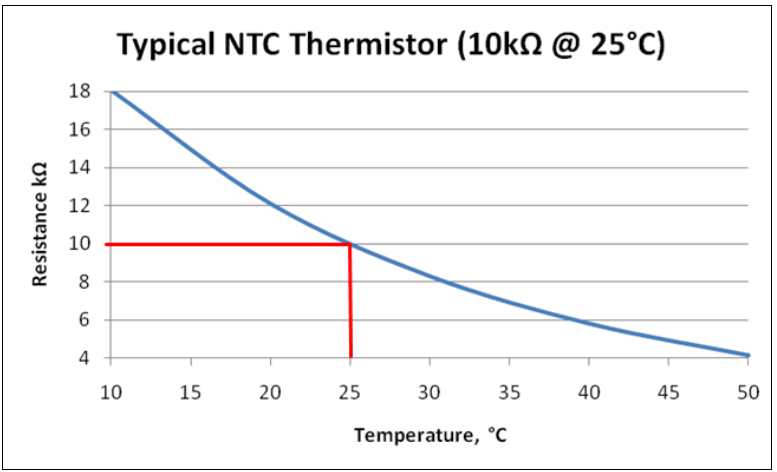
\includegraphics[width=1\linewidth]{images/curva_termistor.png}
				\caption[Curva de resposta típica em termistores NTC de 10k$\Omega$]{Curva de resposta típica em termistores NTC de 10k$\Omega$\footnotemark}
				\label{fig:curva_termistor}
			\end{center}
		\end{figure}
	
		\footnotetext{Fonte: http://www.squids.com.br/arduino/index.php/projetos-arduino/projetos-squids/basico/159-projeto-42-comparando-sensores-de-temperatura-ntc-10k-dht11-e-lm35}


	\subsection{O efeito de Autoaquecimento}

		Como toda resistência, o termistor dissipa energia elétrica na forma de calor. Portanto, ao aplicar uma corrente no sensor, é induzido um efeito de autoaquecimento. A relação da potência elétrica dissipada é dada pela equação \ref{eq:potenciaeletrica} e a relação entre potência e temperatura pode ser obtida através da equação \ref{eq:potenciatermica}. Fazendo $P_E = P_T$, é possível chegar à equação \ref{eq:temperaturacomautoaquecimento}. 
		
		\begin{equation}\label{eq:potenciaeletrica}
			P_E = I.V
		\end{equation}
		sendo:
		\begin{itemize}
			\item $P_E$: Potência elétrica dissipada;
			\item $I$: Corrente elétrica;E
			\item $V$: Tensão entre os terminais.
		\end{itemize}

		\begin{equation}\label{eq:potenciatermica}
			P_T = K(T_{(R)} - T_0)
		\end{equation}
		sendo:
		\begin{itemize}
			\item $P_T$: Potência;
			\item $K$: Fator de dissipação do termistor;
			\item $T_{(R)}$: Temperatura em função da resistência;E
			\item $T_0$: Temperatura ao redor do termistor.
		\end{itemize}
		
		\begin{equation} \label{eq:temperaturacomautoaquecimento}
			T_0 = T_{(R)} - \dfrac{V^2}{K.R}
		\end{equation}
		

\section{A evolução do circuito}

\subsection{O divisor resistivo}
 
Valendo-se da propriedade logarítmica do termistor, uma pequena variação de temperatura ambiente ocasionada pelo processo de expiração ocasionaria uma mudança exponencial no valor da resistência. Por esse motivo, na origem do projeto, era esperada uma medição simples, obtida através da variação de tensão em um divisor resistivo composto por um termistor e uma resistência padrão(Figura: \ref{fig:divisorResistivo}). Contudo, devido alguns contratempos práticos, diversas mudanças fizeram-se necessárias. 
 
Uma das principais limitações para o desenvolvimento do projeto deve-se à dificuldade na aquisição dos componentes eletrônicos que, quando comprados via internet, necessitavam de um tempo para entrega relativamente alto e, para a compra realizada diretamente na loja física, existe uma limitação na variedade de lojas especializadas na cidade do Rio de Janeiro. Outra complicação relevante é referente à ausência de datasheet, que não é informado no momento da compra e torna-se impossível inferir qual é o datasheet correto apenas observando o componente, que é muito pequeno, sem qualquer informação sobre o fabricante ou o modelo. Dadas essas condições iniciais, foi construído o primeiro divisor resistivo apenas com base na informação de que o sensor adquirido tratava-se de um termistor NTC (do inglês Negative Temperature Coefficient) com resistência em temperatura ambiente de $10K\Omega$. Foi utilizada uma fonte de alimentação comercial de $12V$ e utilizado diversos valores entre $10K\Omega$ e $330\Omega$ para a resistência $R2$, contudo para nenhum valor de $R2$ era observada qualquer alteração de tensão na medida em que o ar era exalado próximo ao sensor, contrariando ao que era esperado, dado que a queda de tensão em cima do termistor deve ser variável junto à alteração na resistência.
 
\begin{figure}[h!]
	\begin{center}
 		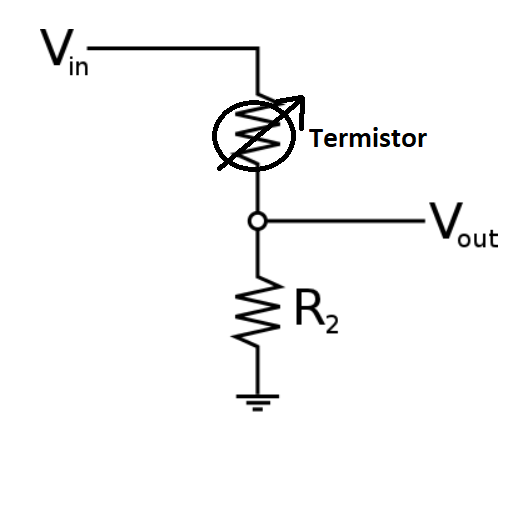
\includegraphics[width=0.5\linewidth]{images/divisor_resistivo.png}
 		\caption{Divisor Resistivo}
 		\label{fig:divisorResistivo}
 	\end{center}
\end{figure}
 
\subsection{Lei de resfriamento de Newton} 
 
A lei de resfriamento de Newton (\ref{eq:resfriamento}) indica que a taxa com que um corpo perde calor é proporcional à diferença de temperatura entre o corpo e o meio  no qual ele se encontra. Valendo-se desse princípio, nota-se que uma baixa diferença de temperatura resultaria em um maior tempo de resposta do sensor. 
 
  
\begin{equation} \label{eq:resfriamento}
	\dfrac{dQ}{dt} = h.A.(T(t) - T_{env}) = h.A \Delta T(t)	
\end{equation}
Onde:
\begin{itemize}[label=]
	\item $Q$: Energia térmica
	\item $t$: Tempo
	\item $h$: Coeficiente de transferência de calor
	\item $A$: Área de transferência de calor
	\item $T$: Temperatura do objeto
	\item $T_{env}$: Temperatura do ambiente
\end{itemize}
 
\begin{equation} \label{eq:autoAquecimento}
	T_0 = T(R) - \dfrac{V^2}{KR}
\end{equation}
Onde:
\begin{itemize}[label=]
	\item $T_0$: Temperatura do meio
 	\item $T(R)$: Temperatura do termistor em função de sua resistência
 	\item $V$: Diferença de potencial entre os terminais do termistor
 	\item $K$: Fator de dissipação do termistor
 	\item $R$: Resistência
\end{itemize}
 
\subsection{Medição da variação do Termistor}

Para entender melhor o comportamento do termistor e a forma com que ele variava sua resistência devido o efeito do autoaquecimento, sem acesso ao datasheet do mesmo, foram realizadas medições utilizando o divisor resistivo, colocando o termistor em série com um resistor fixo de $330\Omega$ e uma fonte de bancada com fornecimento de tensão variável entre $0V$ e $30V$. A curva de variação pode ser observada no gráfico da figura \ref{fig:variacao_termistor}.

\begin{figure}[h!]
	\begin{center}
		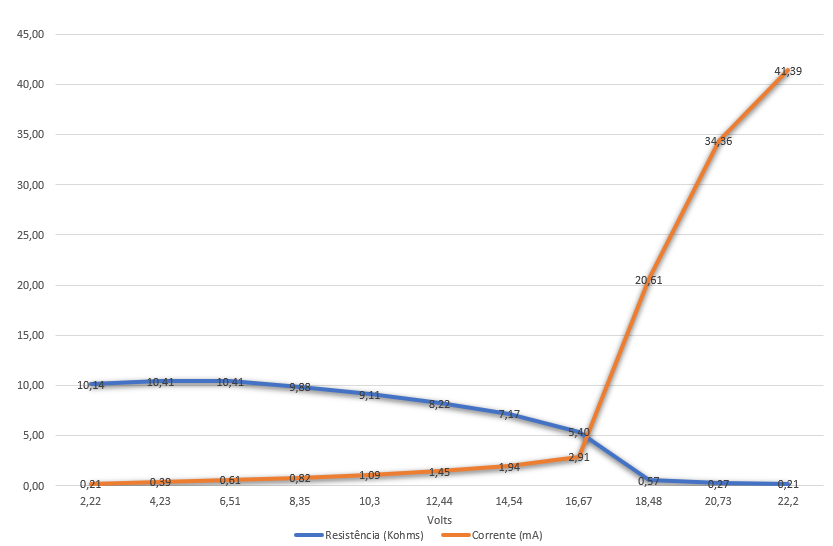
\includegraphics[width=1\linewidth]{images/variacao_resistencia_termistor.png}
		\caption{Variação do termistor em função da tensão}
		\label{fig:variacao_termistor}
	\end{center}
\end{figure}


\subsection{Circuito utilizando o efeito do autoaquecimetno}

Portanto, para contornar o problema obtido devida a lei de resfriamento de Newton, o circuito foi ajustado para utilizar a propriedade de autoaquecimento do termistor (\ref{eq:autoAquecimento}).  
 
Ao aplicar uma alta corrente no sensor, é induzido então um aumento na temperatura deste. Em decorrência desse aumento, é possível observar uma maior diferença de temperatura entre o sensor e o fluxo de ar e, por conseguinte, uma maior taxa para transferência de calor e um menor tempo de resposta por parte do termistor. Contudo, para atingir uma faixa de temperatura sensível, capaz de gerar uma resposta visível ao expor o sensor à respiração, o circuito necessita de uma tensão elevada, acima das entregues por fontes comerciais padrão, que costumam variar entre $5V$ e $12V$, gerando a necessidade de projetar um retificador de tensão capaz de converter a tensão de corrente alternada entregue pela rede elétrica residencial em uma tensão contínua alta o suficiente para fornecer ao termistor a corrente demandada.
 
Realizando testes de bancada, com um gerador de tensão variando de $0V$ à $30V$ e uma resistência de $330\Omega$ em série com o termistor, foi possível atingir uma temperatura sensível ao sopro, entretanto, ao aplicar uma tensão em torno de $22V$, o sensor demorava um tempo considerável para aquecer novamente, tornando-o inviável para medir o comportamento respiratório dada a frequência do sopro em uma respiração normal. Aumentando a tensão para $28V$, já era possível observar uma atenuação considerável na queda constante da temperatura dado que o termistor era capaz de se aquecer mais rápido. O problema gerado por esse aumento de tensão deve-se ao fato de que, quanto maior é a corrente, maior é o autoaquecimento e, quanto maior a temperatura, menor é a resistência, gerando um aumento ainda maior na corrente passante que, por sua vez, aumenta ainda mais a temperatura até que o sensor atingia um patamar no qual queimava, caso não houvesse nenhum sopro forçando a temperatura a diminuir. 
 
Para suprir o fornecimento de tensão em corrente contínua em torno dos $28V$ foi necessário construir um retificador de tensão, uma vez que as fontes padrão, encontradas no mercado, costumam fornecer tensão menor que a desejada.

-- Colocar foto do circuito e do projeto da fonte 
 
\subsection{Circuito com controle realimentado} 
 
Se por um lado, o aumento da tensão era importante para que a temperatura não decaísse constantemente ao iniciar a medição respiratória, por outro, o sistema precisava ser protegido para que a corrente não atingisse um determinado patamar que danificasse o componente. O ajuste mais simples para regular a corrente em um componente costuma ser adicionar uma resistência em série, diminuindo a corrente por uma mera consequência da lei de ohm (\ref{eq:leideohm}). Contudo, por se tratar de uma resistência variável, a tensão necessária para o aquecimento do termistor em seu estado inicial era maior que a tensão necessária para mantê-lo abaixo de um patamar seguro após a diminuição de sua resistência pelo efeito do autoaquecimento. Foi pensado então em um circuito de controle não linear (Figura: \ref{fig:circuitoRealimentado}), que, em teoria, forneceria uma alta tensão para o termistor até que sua resistência variasse e a corrente passante atingisse um patamar determinado. 
  
\begin{equation} \label{eq:leideohm}
	V = R.I
\end{equation}
Onde:
\begin{itemize}[label=]
  	\item $V$: Tensão
  	\item $R$: Resistência
  	\item $I$: Corrente
\end{itemize}

\begin{figure}[h!]
	\begin{center}
		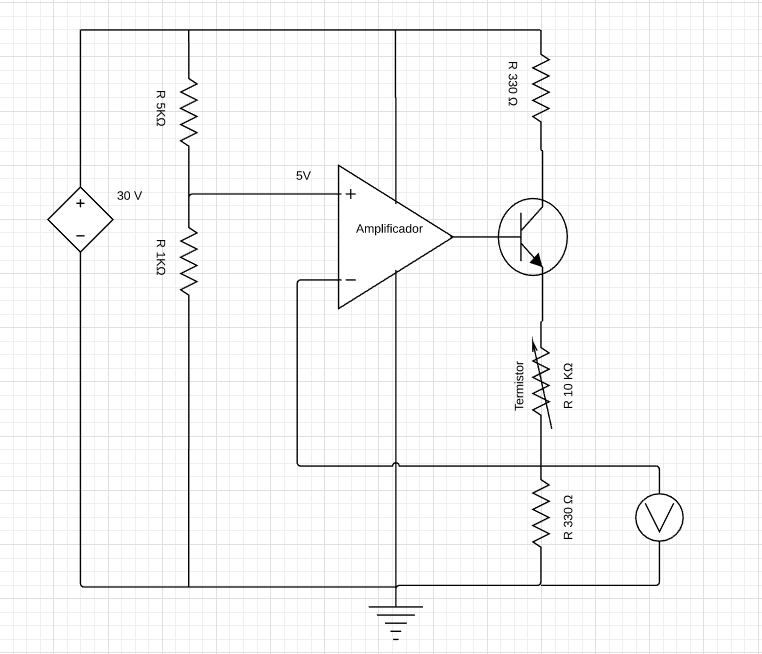
\includegraphics[width=1\linewidth]{images/Circuito_de_controle.png}
		\caption{Circuito de Controle}
		\label{fig:circuitoRealimentado}
	\end{center}
\end{figure}

O comportamento esperado para o circuito de controle seria o seguinte: O amplificador operacional iria ajustar a tensão de saída na tentativa de igualar as tensões nos dois terminais de entrada, sendo assim, no momento inicial, quando a tensão no terminal de entrada negativo é igual a zero e a do terminal positivo é igual a $5V$, o amplificador aumenta sua saída fazendo com que o transistor entre em saturação e conduza uma corrente no emissor praticamente igual à de referência no coletor, na medida em que a resistência do termistor diminui pelo efeito de autoaquecimento, a tensão de saída aumenta até que esta se iguale à do terminal positivo, ao atingir esse patamar, o transistor sai da zona de saturação e o sistema trabalha pra manter a tensão de saída constante. No momento em que o sensor entra em contato com o fluxo de ar, a resistência do termistor aumenta, diminuindo a tensão na saída e estimulando o sistema de controle a saturar o transistor e induzir o efeito do autoaquecimento no sensor. Após quantizar a tensão da saída através de um microcontrolador, foi possível traçar o gráfico da figura \ref{fig:RespostaCircuitoRealimentado}, no qual aparece nítida a resposta do sistema ao submeter o sensor a um fluxo de ar. Entretanto, ao expor o sensor a um período prolongado de exposição à respiração humana, foi possível observar que o efeito do resfriamento contínuo continuava a ser reproduzido (gráfico da figura \ref{fig:RespostaCircuitoRealimentadoLongoPrazo}).


\begin{figure}[h!]
	\begin{center}
		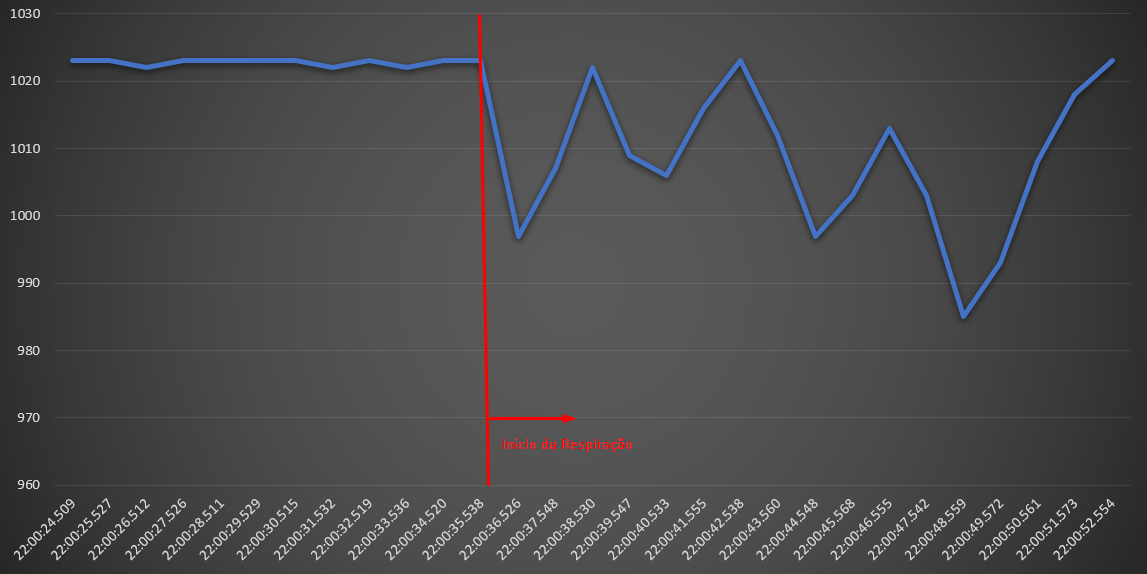
\includegraphics[width=1\linewidth]{images/RespostaCircuitoRealimentado.png}
		\caption{Resposta em curto prazo circuito realimentado (Tempo no eixo horizontal e valor de tensão quantizado no eixo vertical)}
		\label{fig:RespostaCircuitoRealimentado}
	\end{center}
\end{figure}

\begin{figure}[h!]
	\begin{center}
		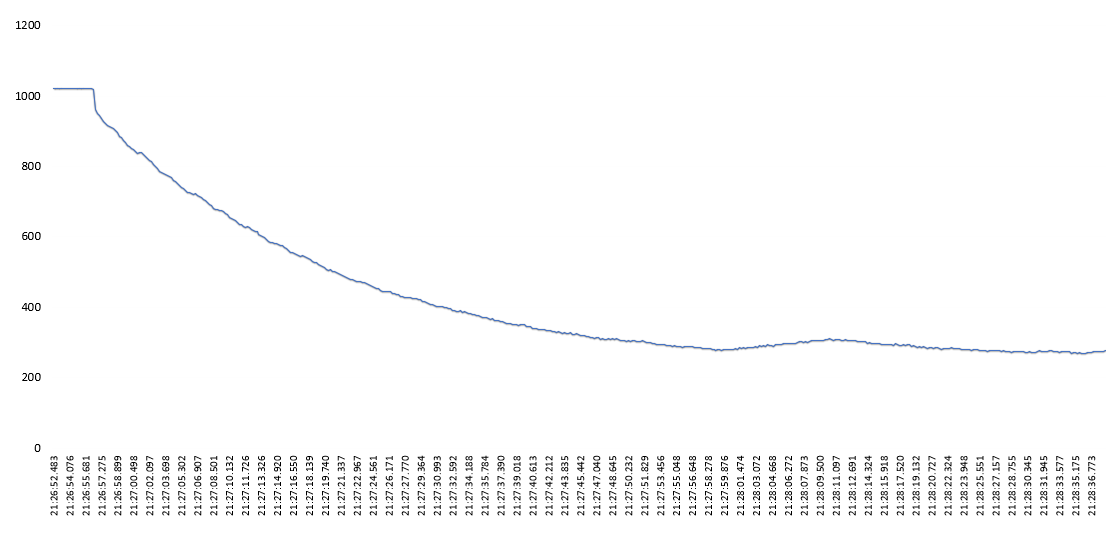
\includegraphics[width=1\linewidth]{images/DecaimentoRespiracaoMascara.png}
		\caption{Resposta de longo prazo circuito realimentado (Tempo no eixo horizontal e valor de tensão quantizado no eixo vertical)}
		\label{fig:RespostaCircuitoRealimentadoLongoPrazo}
	\end{center}
\end{figure}
\FloatBarrier



 
 
\section{O Software}

Em paralelo ao desenvolvimento do hardware, foi desenvolvido um software capaz de obter os dados de um microcontrolador através de uma porta serial no computador. Dada a escolha do Arduíno para o desenvolvimento do protótipo de baixo custo, era possível abstrair o desenvolvimento do hardware pressupondo, de antemão, que o circuito deveria ser projetado para entregar à entrada analógica do Arduíno um sinal de tensão variante entre $0V$ e $5V$. Para interpretar esse sinal, o microcontrolador existente no Arduíno (ATmega328) converte o sinal analógico em digital. A resolução do sinal convertido é dada pela equação \ref{eq:resolucaoArduino}, sendo o valor da tensão de referência igual a $5V$ e a quantidade de bits disponível para conversão igual a $10bits$, chegamos a uma resolução de $4,48mV$. Em outras palavras, abstraindo do hardware, o software deveria ser programado para ser capaz de receber uma entrada pela porta serial e ler sinais inteiros variando entre  $0$ e $1024$ (Equivalente a $10bits$) onde cada variação inteira representa $4,48mV$ do sinal de entrada do Arduíno.


\begin{equation} \label{eq:resolucaoArduino}
	Resolucao = \dfrac{V_{ref}}{2^n}
\end{equation}
Onde:
\begin{itemize}[label=]
	\item $V_{ref}$: Tensão de referência
	\item $n$: Número de bits do conversor
\end{itemize} 

A linguagem de programação escolhida para o desenvolvimento do software foi o Python dada a sua notória ascensão e eficiência para a realização de operações matemáticas e tratamento de dados científicos, além de ser referência em áreas como inteligência artificial (o que viabilizaria estudos futuros nessa área).

\subsection{Software de teste de conceitos}

\subsubsection{Leitura do sinal de entrada} \label{sub:LeituraSinalEntrada}


Antes de gerar um sinal simulado para iniciar o efetivamente o desenvolvimento do software, foi desenvolvido um pequeno protótipo para garantir que seria possível a comunicação entre um sinal gerado pelo Arduíno e o software desenvolvido em Python. Basicamente, existem dois softwares atuando simultaneamente para realizar essa leitura. Um, desenvolvido na linguagem de programação C, que fica instalado diretamente no Arduíno e é responsável por realizar a medição periódica e crua do sinal digital, logo após a sua quantização, e escrever um par valor x tempo na porta USB. O segundo é, de fato, o programa escrito em Python que, dentre outras funções realiza a leitura do sinal escrito pelo programa anterior na porta USB e salva os dados em um arquivo .csv, que poderá ser lido futuramente para a realização das operações matemáticas.


\begin{figure}[h!]
	\begin{center}
		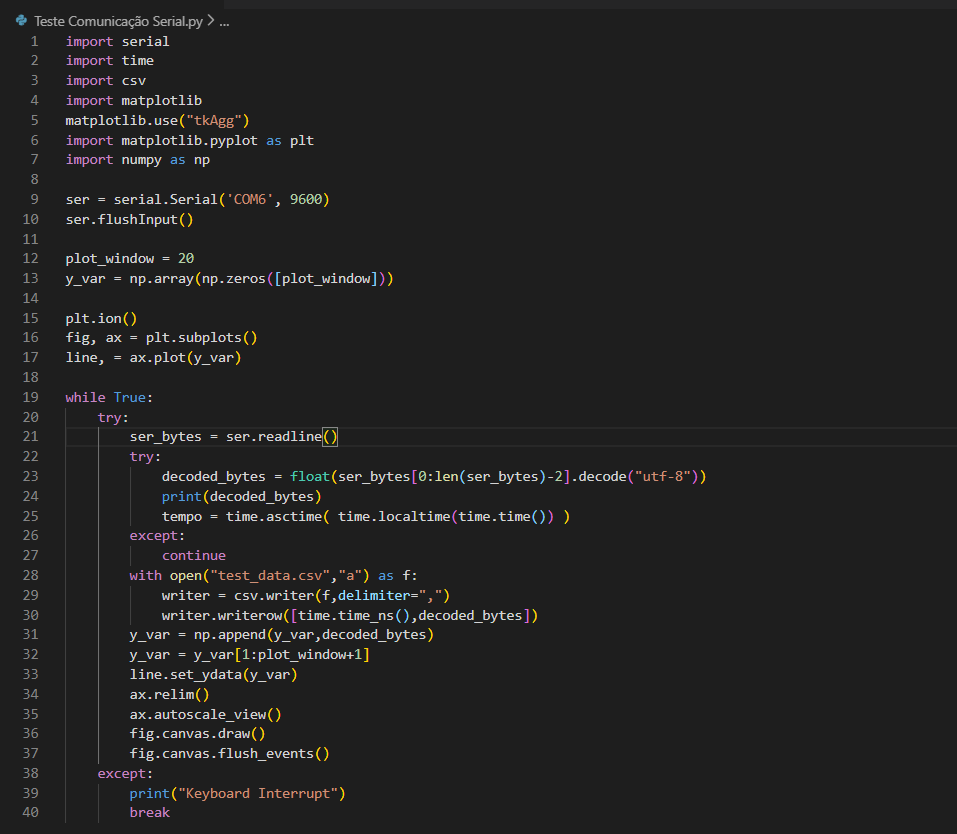
\includegraphics[width=1\linewidth]{images/LeitorDeUSB.png}
		\caption{Leitor de porta USB}
		\label{fig:LeitorDeUSB}
	\end{center}
\end{figure}


\subsubsection{Simulação do sinal de entrada}

Durante os experimentos com o hardware, foi possível observar um padrão na resposta do sinal analógico quando medido pelo osciloscópio que, em todas as versões do circuito, possuía um comportamento muito similar (imagem \ref{fig:ComportamentoSinalAnalogico}). A forma desse sinal pode ser explicada observando o princípio de funcionamento escolhido para que o sensor de temperatura seja capaz de medir a respiração. Em um cenário ideal, espera-se que o sensor esteja aquecido até que encontre uma temperatura de equilíbrio de operação e, quando em contato com um fluxo de ar da inspiração ou expiração, essa temperatura irá diminuir, aumentando a resistência do sensor e, em consequência, exibindo, no osciloscópio, uma diminuição da tensão. Quando acaba o fluxo de ar (tempo entre a expiração e inspiração), o circuito tentará esquentar novamente o sensor até que ele retorne à temperatura de equilíbrio. É possível também, observar que possuímos duas faixas distintas de amplitude na queda de tensão, o que nos faz concluir que o sensor tenderá a não obter uma resposta indiferente ao tipo de fluxo de ar (inspiração ou expiração) seja pelo fato de que a temperatura do ar na expiração é levemente maior, ou seja devido à construção que pode privilegiar o contato do fluxo do ar com o sensor em um sentido mais que no outro. Nos casos experimentados até então, por exemplo, a queda de tensão decorrente da inspiração era consideravelmente maior que a da expiração.


\begin{figure}[h!]
	\begin{center}
		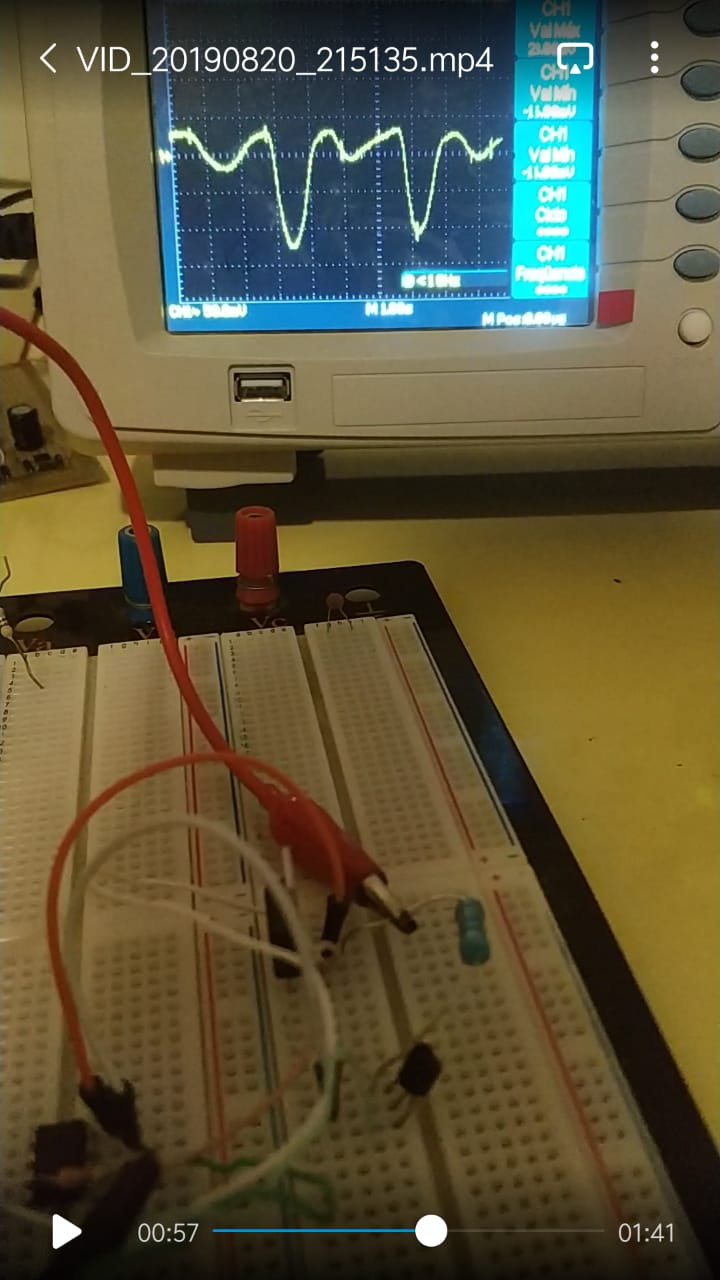
\includegraphics[width=0.5\linewidth]{images/ComportamentoSinalAnalogico.jpeg}
		\caption{Leitura do sinal analógico no osciloscópio}
		\label{fig:ComportamentoSinalAnalogico}
	\end{center}
\end{figure}

Considerando o comportamento dos sinais analógicos obtidos nas versões de circuito anteriores e o caráter cíclico natural do comportamento respiratório, o sinal de entrada foi simulado como um somatório de senoides com diferentes amplitudes e frequências. A frequência escolhida para o sinal principal foi a de 18 ciclos por minuto, que é a faixa superior da frequência considerada confortável para um adulto normal em repouso. Uma nova senoide com a metade da frequência foi gerada e posta defasada de modo a atenuar os picos referentes à expiração e agravar os relacionados à inspiração e, para a simulação do ruído, foi adicionada mais uma senoide com frequência mais elevada. O sinal simulado pode ser descrita conforme a equação \ref{eq:sinalSimulado} e produz o resultado apresentado no gráfico da figura \ref{fig:Funcao_simulada_interpolada}.

\begin{equation} \label{eq:sinalSimulado}
	F(t) =  \sin(0.15 * 2\pi t)  + 0.8\sin(\dfrac{\pi}{2} + 0.3 * 2\pi t) + 0.1\sin(\dfrac{\pi}{2} + 30 * 2\pi t)
\end{equation}


\begin{figure}[h!]
	\begin{center}
		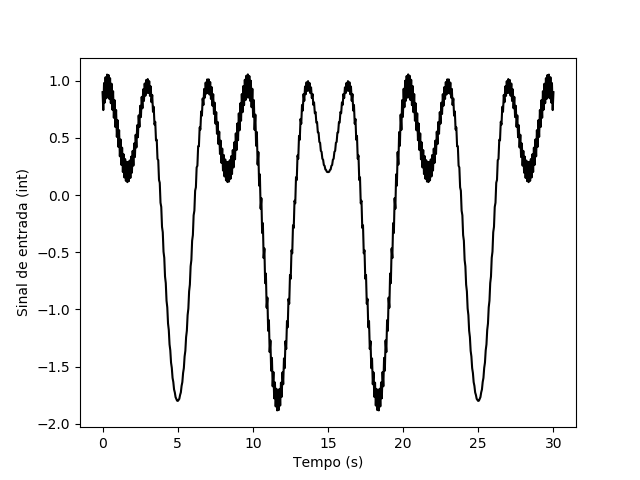
\includegraphics[width=0.5\linewidth]{images/Funcao_simulada_interpolada.png}
		\caption{Função simulada interpolada}
		\label{fig:Funcao_simulada_interpolada}
	\end{center}
\end{figure}



\subsubsection{Operações Realizadas}

A primeira versão do software foi projetada para ser capaz de realizar as seguintes operações:

\begin{itemize}[label=]
	\item 1- Ler os dados de uma porta serial via usb que serão enviados por um arduíno (trecho do código descrito na subseção \ref{sub:LeituraSinalEntrada})     
	\item     2- Criar pastas com o nome e horário das medições para o armazenamento dos arquivos
	\item     3- Salvar os dados em um arquivo .csv     
	\item     4- Ler os dados do arquivo csv e realizar as seguintes operações:     
	\subitem         4.1- Plotar diretamente
	\subitem         4.2- Plotar uma interpolação
	\subitem         4.3- Calcular a derivada primeira e segunda e plotar
	\subitem         4.4- Calcular a FFT e plotar    
	\item     5- Ler o arquivo csv, passar por um filtro IIR passa baixas, salvar um novo csv e realizar as seguintes operações:     
	\subitem         5.1- Plotar diretamente
	\subitem         5.2- Plotar uma interpolação
	\subitem         5.3- Calcular a derivada primeira e segunda e plotar
	\subitem         5.4- Calcular a FFT e plotar     
	\item     6- Ler o arquivo csv, passar por um filtro IIR passa baixas, salvar um novo csv e realizar as seguintes operações:        
	\subitem         6.1- Plotar diretamente
	\subitem         6.2- Plotar uma interpolação
	\subitem         6.3- Calcular a derivada primeira e segunda e plotar
	\subitem         6.4- Calcular a FFT e plotar     	 
\end{itemize} 

\subsubsection{Calculo das derivadas}

Para obter a derivada do sinal de entrada utilizamos o método das diferenças finitas \ref{eq:diferencasFinitas}, uma vez que, ao ser processado pelo programa, o sinal encontra-se discretizado e com uma boa quantidade de pontos devido a alta taxa de amostragem em relação à frequência de variação da tensão provocada pela respiração. O sinal discretizado é armazenado em dois vetores de mesmo tamanho, onde um armazena o valor da tensão e outro o valor do tempo de medição. Ao realizar o somatório da equação \ref{eq:diferencasFinitas} em todos os pontos dos vetores, conseguimos plotar o gráfico da derivada. Foi criada uma função no programa em Python que recebia como parâmetro os vetores x e y e retornava o resultado operação supracitada, permitindo assim o reuso do método para o cálculo da derivada segunda.


\begin{equation} \label{eq:diferencasFinitas}
	f'(x) =  \sum_{X0}^{Xn} \dfrac{f(x+\Delta x) - f(x)}{\Delta x}
\end{equation}
Onde:
\begin{itemize}[label=]
	\item $f'(x)$: Derivada da tensão no ponto x
	\item $X0$: Primeiro valor do vetor de tempo
	\item $Xn$: Último valor do vetor de tempo
	\item $f(x)$: Valor da tensão no ponto x
\end{itemize}

\subsubsection{Fast Fourier Transform (FFT)}

Para obter informações referentes à frequência do sinal respiratório, o sistema calcula e plota um gráfico realizando uma análise de Fourier, convertendo o sinal original, no domínio do tempo, em uma representação no domínio da frequência. Contudo,  realizar o cálculo da transformada de Fourier diretamente de sua definição \ref{eq:DTFT} implica em operações aritméticas de complexidade  \boldmath $O(n^2)$, entretanto é possível atingir o mesmo resultado utilizando a FFT com uma complexidade de apenas $O(n \log (n)) $.   \unboldmath Aumentando a performance do software.



\begin{equation} \label{eq:DTFT}
	\mathcal{F} 	\left \{ f(t) \right \}  = \int_{-\infty}^{\infty} f(t) e^{-j \omega t}\,dt
\end{equation}

\subsubsection{Complexidade de algorítimo}

A complexidade de um algorítimo é determinada através da relação entre o tempo e memória gastos para realizar a operação de acordo com o tamanho da entrada. Ou seja, em termos práticos, é a complexidade do algorítimo, aliada à capacidade de processamento do computador, quem determinará a velocidade de funcionamento do sistema na medida em que se aumenta a quantidade de dados na entrada. A forma mais popular de representar a complexidade de tempo na análise de algorítimos é a \textbf{\textit{complexidade assintótica}}, que ignora fatores constantes e os termos que crescem mais lentamente. Por exemplo, em uma relação onde o tempo de execução $T(N)$ em função da entrada de dados $N$ é de $T(N) = 27N^2 + 45N + 12$, na medida em que $N$ aumenta, a função pode ser simplificada por $T(N) = 24N^2$. Simplificando ainda mais a análise, para prever o quão rápido será o crescimento do tempo de execução em relação ao aumento da entrada, podemos desconsiderar a constante que multiplica o termo de maior grau, uma vez que, tanto para $T(N) = 100000N^2$ quanto para $T(N) = 10N^2$, dobrar a entrada $N$ implicará em quadruplicar o tempo $T(N)$. Representamos $O(g)$ como sendo o limite superior para o tempo gasto por um algorítimo, em outras palavras, $O(g)$ representa a classe de funções que crescem, no máximo, tão rápidas quanto a função $g$. Ou seja, reduzir o cálculo da FFT de complexidade \boldmath $O(n^2)$ para $O(n \log (n)) $.   \unboldmath representa diminuir o tempo de execução, antes limitado pela função em vermelho, para a função em azul no gráfico da figura \ref{fig:grafico_complexidade}.

\begin{figure}[h!]
	\begin{center}
		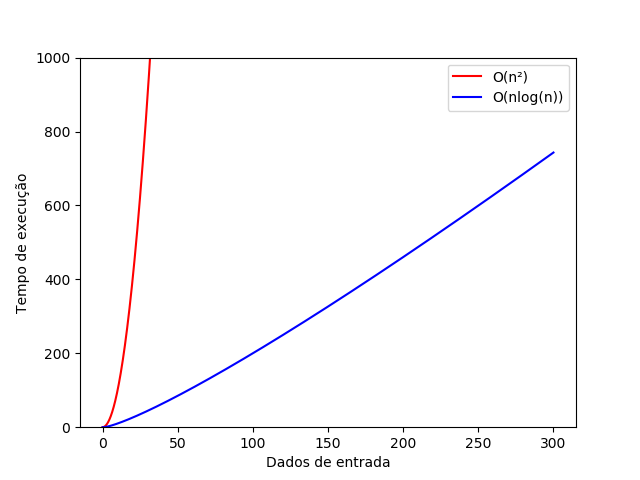
\includegraphics[width=0.7\linewidth]{images/Complexidade_algoritmo.png}
		\caption{Relação entre \boldmath $O(n^2)$ e $O(n \log (n)) $.   \unboldmath}
		\label{fig:grafico_complexidade}
	\end{center}
\end{figure}

\subsubsection{Filtro passa-baixas}

Com a finalidade de eliminar eventuais ruídos, o sistema é capaz de aplicar filtros passa-baixas, eliminando altas frequências ruidosas e preservando as variações que ocorrem em uma faixa de frequência compatível com a respiração humana (abaixo de 70 ciclos por minuto em atletas). Os filtros digitais são divididos em duas classes FIR e IIR e, para maior liberdade do pesquisador, o sistema oferece as duas opções de filtragem.

\subsubsection{IIR (Infinite Impulse Response)}

Os filtros IIR são mais rápidos que os FIR. Para esse programa, foi escolhido o filtro de Butterworth, que possui resposta na frequência conforme a figura \ref{fig:Filtro_Butterworth}. Na medida em que aumentamos a ordem do filtro, conseguimos obter uma atenuação mais ingrime na filtragem \ref{fig:Ordem_Filtro_Butterworth}, contudo, adicionamos mais complexidade ao cálculo. Para o experimento, foi escolhida, empiricamente, o filtro de ordem 3. Chamamos de frequência de corte a frequência na qual o sinal possui atenuação de $-3 dB$ e esta foi escolhida de forma a permitir que o sinal na banda de frequências da respiração fosse preservado.

\begin{figure}[h!]
	\begin{center}
		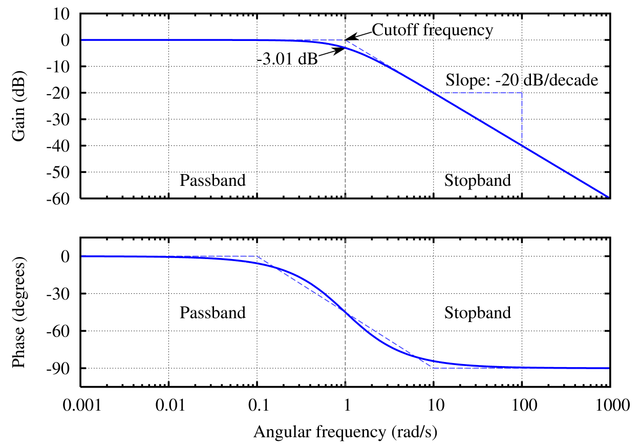
\includegraphics[width=0.7\linewidth]{images/Butterworth_filter_bode_plot.png}
		\caption{Resposta de um filtro Butterworth}
		\label{fig:Filtro_Butterworth}
	\end{center}
\end{figure}

\begin{figure}[h!]
	\begin{center}
		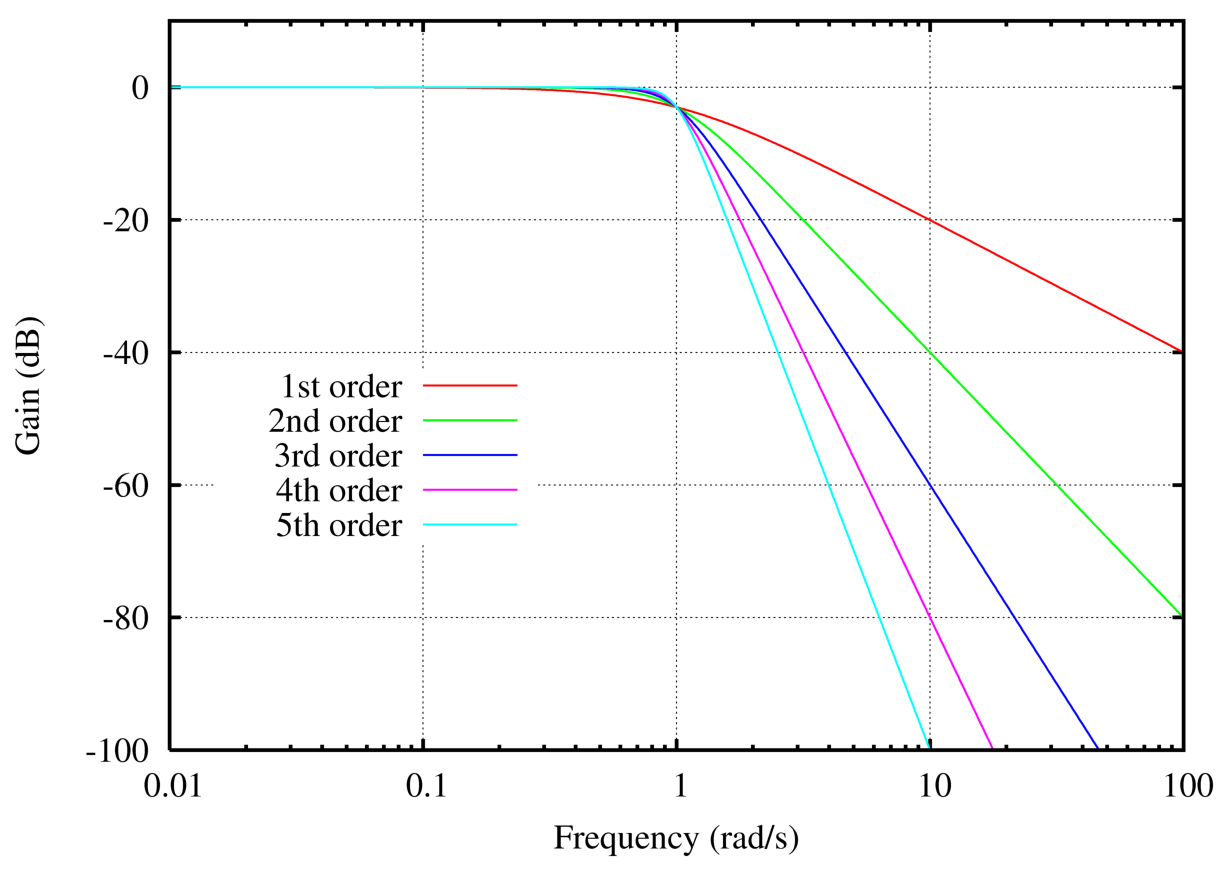
\includegraphics[width=0.5\linewidth]{images/Butterworth_orders.png}
		\caption{Resposta de um filtro Butterworth}
		\label{fig:Ordem_Filtro_Butterworth}
	\end{center}
\end{figure}

\subsubsection{FIR Finite Impulse Response}

A implementação do filtro FIR foi realizada utilizando o método de janelas. Nessa primeira fase do projeto, foi utilizada a janela de Hamming, que é definida pela equação \ref{eq:Hamming} e possui resposta em frequência conforme a figura \ref{fig:Janela_Hamming}.
 
 
\begin{equation} \label{eq:Hamming}
w(n) = 0,54 - 0,46\cos \left(\dfrac{2\pi n}{M - 1}\right) \qquad 0 \le n \le M-1
\end{equation} 

\begin{figure}[h!]
	\begin{center}
		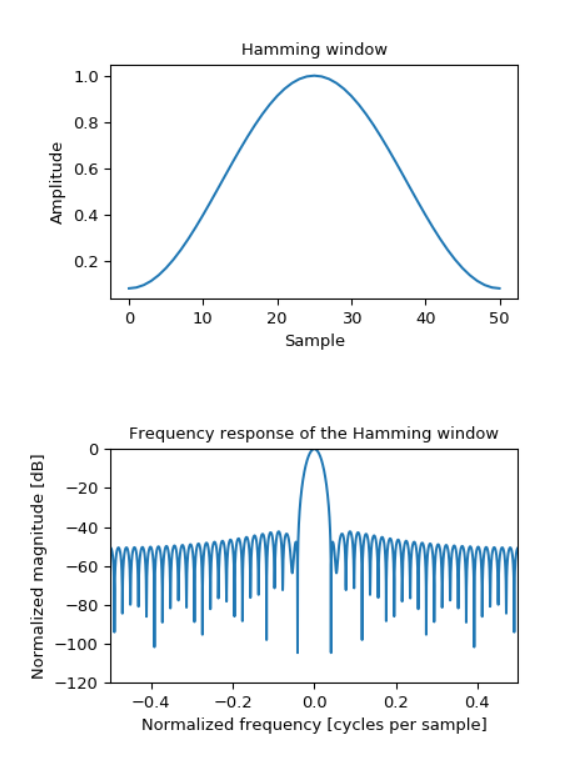
\includegraphics[width=1\linewidth]{images/janela_de_hamming.png}
		\caption{Resposta de uma janela de hamming}
		\label{fig:Janela_Hamming}
	\end{center}
\end{figure}

\subsection{Evolução do software para um sistema web}

\subsubsection{Flask}
\subsubsection{MongoDB}
-- Ou separar por telas
\subsubsection{upload de arquivo csv}
\subsubsection{Validação de CPF}
 